\subsection{Modularity}

A Software module can be defined as self-contained units of code that perform specific
tasks or sets of tasks within a larger system. A software module is designed to operate
independently of other modules, with well-defined interfaces that allow it to communicate
and exchange data with other modules if necessary \autocite[22]{mannaert_normalized_2016}.

A module can be considered a hierarchical and recursive concept. They are independent of
their size (lines of code) or computational magnitude. They can be as small as a function
as part of a class. The class itself can also be considered a module. A group of classes
contained in a Dynamic Link Library (DLL) or Application Programming Interface (API) can
also be considered a module of an even bigger system. 

An important part of the design of a software system is to identify the possible different
modules and their interaction interfaces. Figure \ref{fig:modulair_components} presents a
high-level depiction of modular manifestations in the artifact, with additional examples
of modularity found in more granular implementations. Further discussion of this
architecture is provided in Chapter \ref{sec:ca_theory}.

\begin{figure}[H]
    \centering
    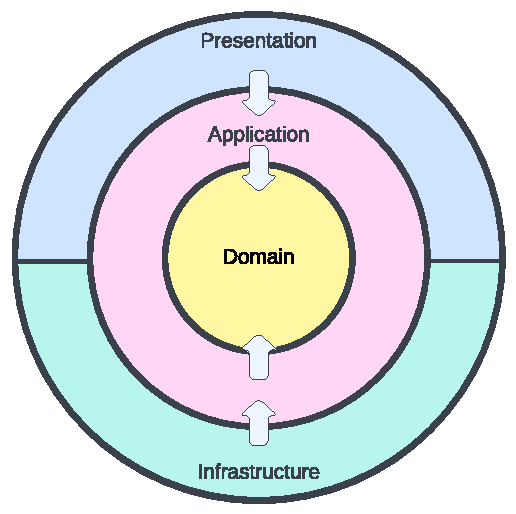
\includegraphics[width=0.4\textwidth]{Figures/ca_diagram.pdf}
    \caption[modularity]{The modular components of the artifacts.}
    \label{fig:modulair_components}
\end{figure}